\subsubsection{Exercise}

Using the method depicted in Exercice \ref{exo411} with $\tau_I = 1$s places the integral action too close to the cross-over frequency: The lag-action and the lead-action of the controller are overlapping.

Therefore, we increase the value of $\tau_I$ to $\tau_I = 10$s and apply the same method as in Exercice \ref{exo411} to get the values of $\tau_D$ and $\beta$.

The resulting controller fulfill all the criteria. (see Figure \ref{figbode413} and \ref{figstep413}).

The lead lag controller with a phase-margin of $50^{\circ}$ has the following caracteristics:
\begin{center}
\begin{tabular}{|c|c|}
    \hline
    Bandwith ($-3dB$) & $[0,0.99]$(rad/s)\\
    \hline
    Resonance peak $M_T$ & $2.06$dB at $0.56$(rad/s)\\
    \hline
    Rise time $t_r$ & $2.22$ s\\
    \hline
    Overshoot $D$\% & $15.7$\%\\
    \hline
\end{tabular}
\end{center}

\begin{figure}[h!t]
   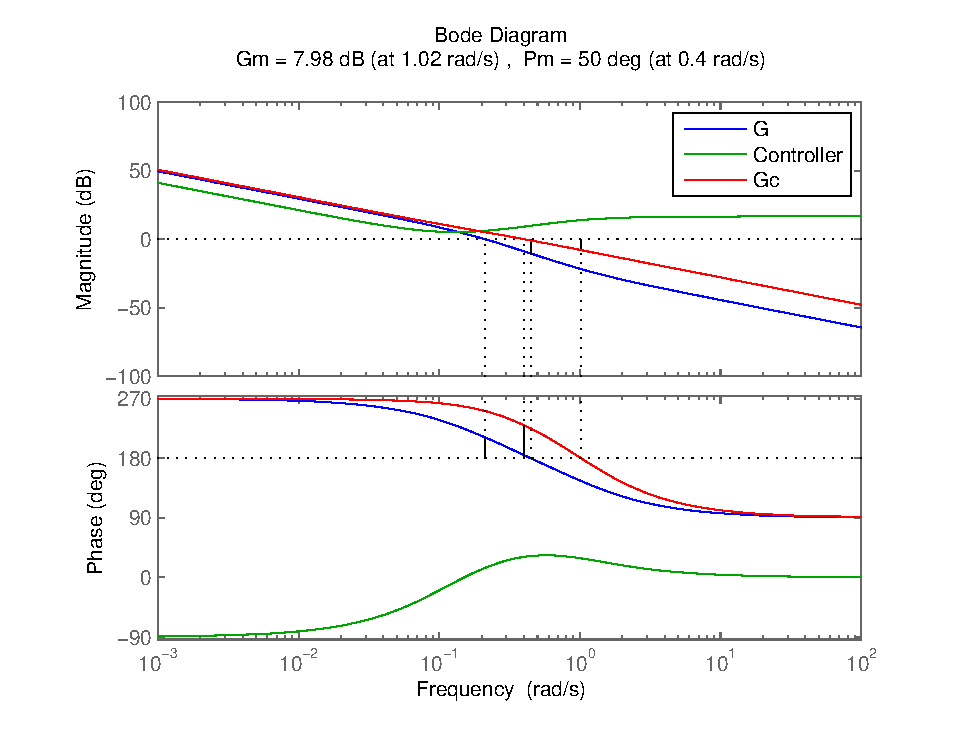
\includegraphics[width=\columnwidth]{fig/bode413.eps}
    \caption{Bode diagram of the system's functions \\ Phase-margin: $50^{\circ}$} 
    \label{figbode413}
\end{figure}

\begin{figure}[h!t]
   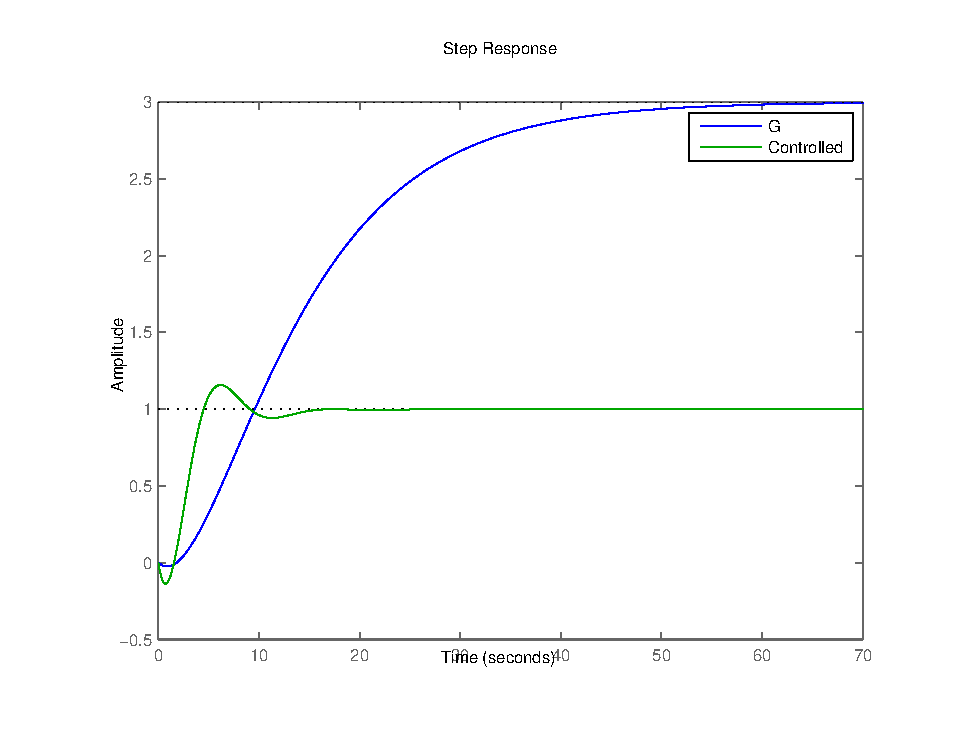
\includegraphics[width=\columnwidth]{fig/step413.eps}
    \caption{Step response of the system with and without the controller \\ Phase-margin: $50^{\circ}$}
    \label{figstep413}
\end{figure}



